\section{Usage}\label{Usage}
This section will describe the systems interaction with its surroundings. This will be done by making an actor specification and then presenting user pattern diagrams, which will be showcased in state machine diagrams.

\subsection{Actor specification}
\label{Actor_specification}
This system only contains one actor, which is the user of the system. The actor will be described by an actor specification.

\textbf{Objective:} A person who prepares meals, either for himself or for a household. The user's primary need is to plan his week in order to efficiently shop groceries and reduce food waste.

\textbf{Characteristic:} The system includes a user base of which the users have different needs and preferences.

\textbf{Example one:} User A is allergic to nuts and has to make meals which excludes these. When he is shopping he needs to look at the package info to make sure that the product does not contain traces of nuts.

\textbf{Example two:} User B is a young student who is in a relationship. He has a tight budget and a short time frame to shop in. The couple finds it difficult to sustain an overview of their shared storage of food. Therefore User B will sometimes buy products the couple do not need, for example, he might purchase milk even though they already have three litres stored. This will sometimes result in them not being able to use all the milk before it expires, which is bad for their shared budget and food waste.



\subsection{Use Cases}
The use cases shows how the actor interacts with the system to complete tasks. These interactions are shown in state machine diagrams. The diagrams show how the dynamic states can shift through interactions with the actor. Even though many of the details is excluded, it still gives an overview of the logic and flow behind the use cases.

The purpose of the diagram is to create an overview of the application domain's interactions with the system. This will be used to find requirements for the functions and user interface. There are three user pattern diagrams, each representing different areas of the system. The three diagrams showcase the user patterns in the:

\begin{itemize}
\item{Shopping list}
\item{Meal plan}
\item{Inventory}
\end{itemize}

When the user navigates the system, the user will undertake one of two roles. An administrative or a planning oriented role.
The option to go back or cancel have not been included in any of the diagrams, as their only contribution is to make the diagrams less readable and add redundant repetitions.

\Cref{Foodplan_Figure} shows the state machine diagram for planning meals. In this part of the system the user operates under the role of planning.

\begin{figure}[H]
	\centering
	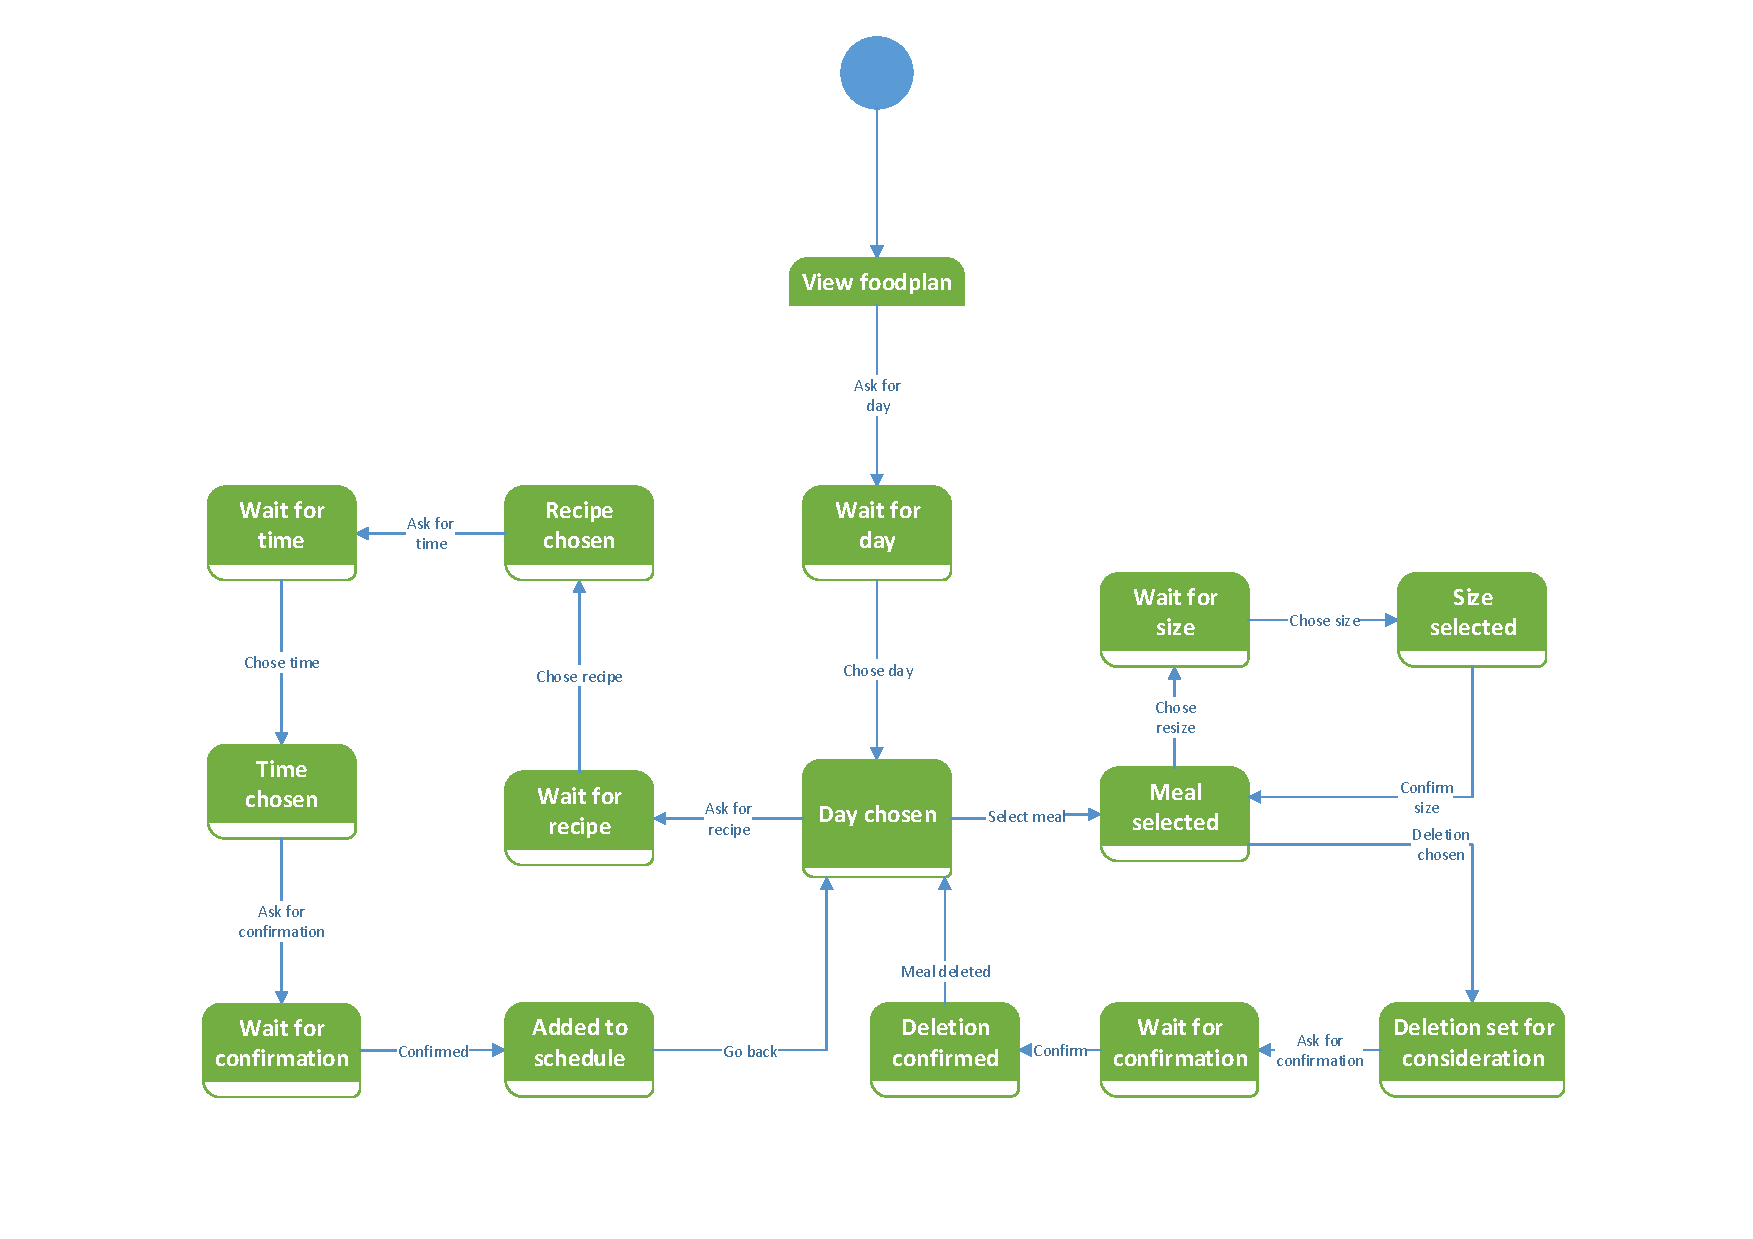
\includegraphics[width=1.0\textwidth]{ApplicationDomain/spViewFoodPlan.pdf} 
	\caption{State machine diagram for meal planning.}
	\label{Foodplan_Figure}
\end{figure}
When the user navigates to the meal plan part of the system, he will have to choose a day to view the meal plan for. From there the user can add a new meal to the plan or select an existing planned meal. If the user chooses to add a new meal, the system will ask for a recipe. The recipes the user can choose from varies depending on the user's preferences. If the user has chosen to avoid some products, recipes that contain those products will be excluded. When a recipe has been chosen, a time can be entered for when the meal should be prepared. After confirmation the meal will be added to the schedule.

The next two diagrams, \cref{Inventory_Figure} and \cref{spEditInventory}, are for the inventory. In this part of the system the user operates as an administrator.

\begin{figure}[H]
	\centering
	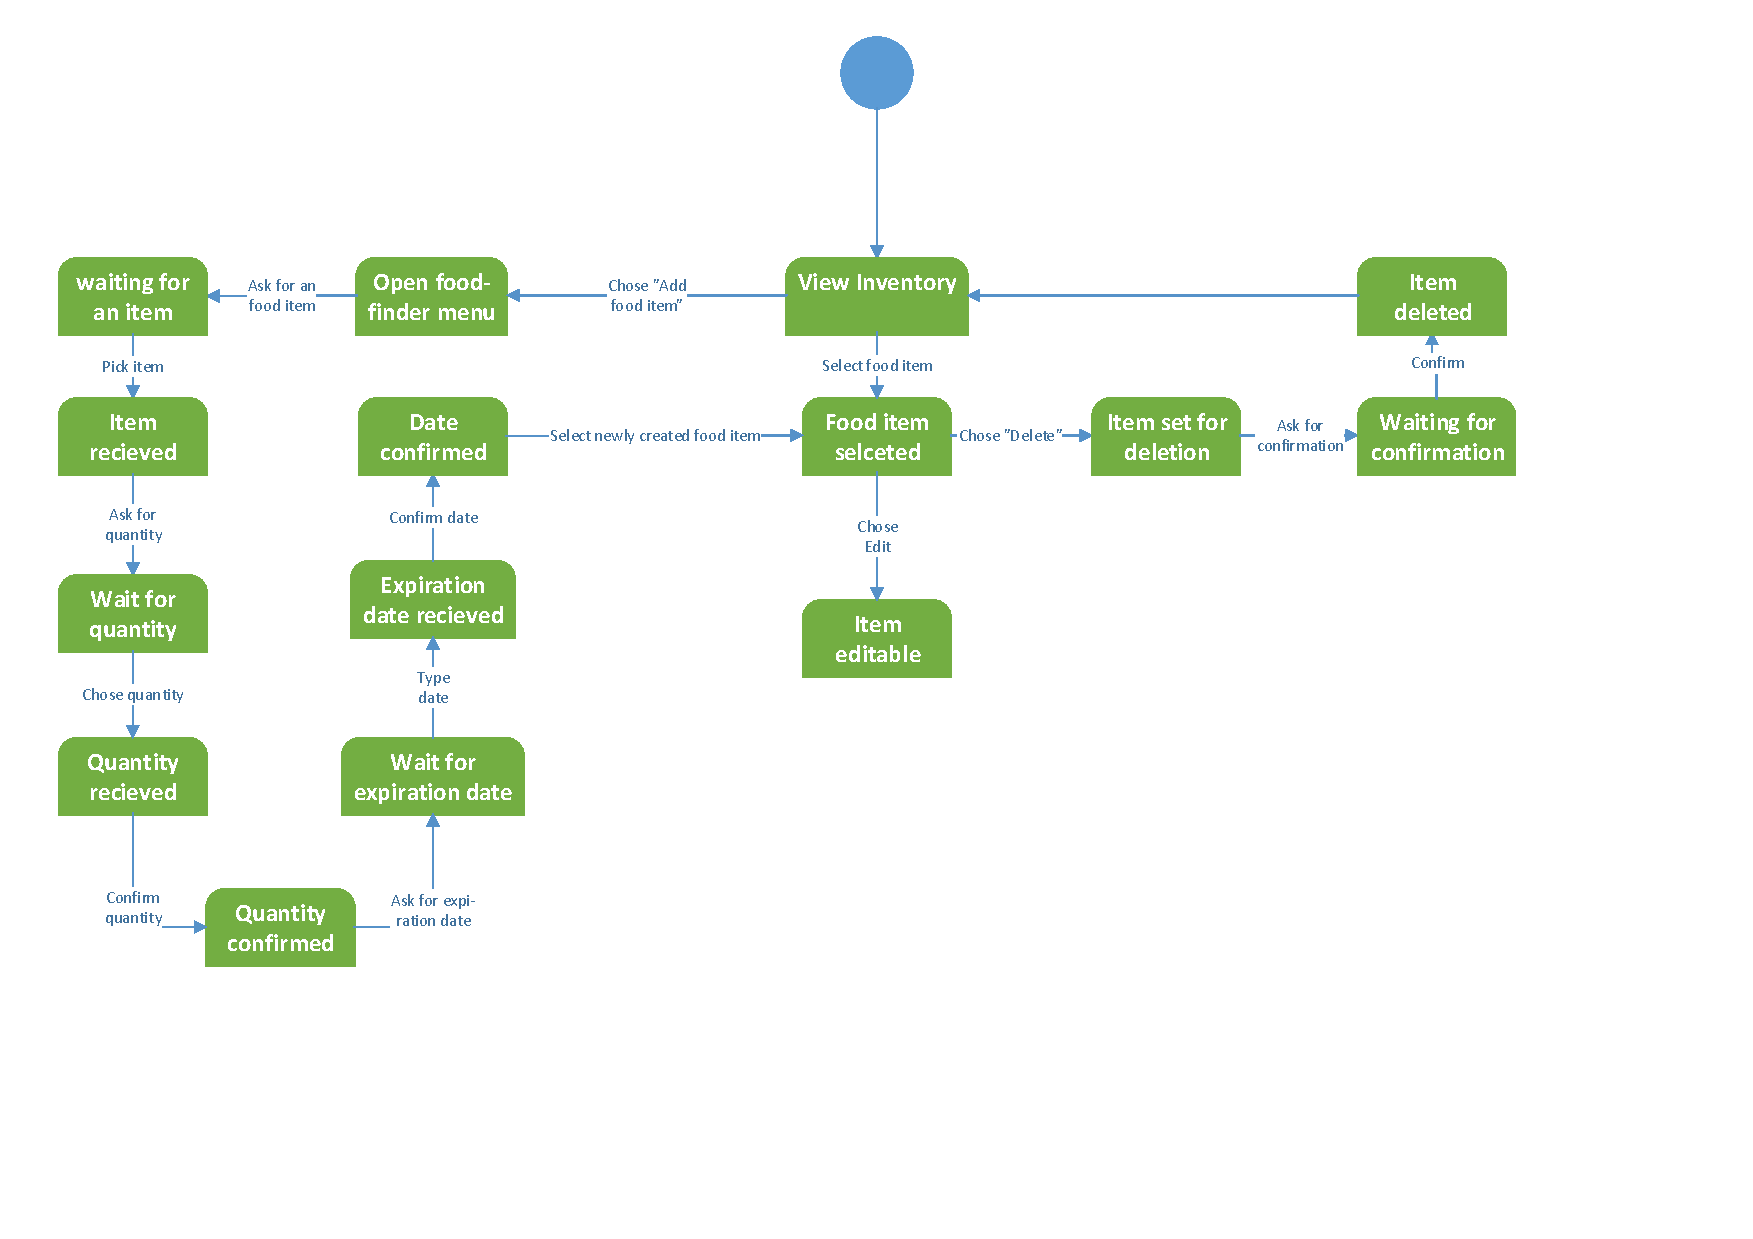
\includegraphics[width=1.0\textwidth, trim= 0 4cm 3cm 0]{ApplicationDomain/spViewInventory.pdf} 
	\caption{The \textit{View Inventory} state diagram}
	\label{Inventory_Figure}
\end{figure}
The user starts on the \textit{View Inventory} state where the inventory is shown. From here the user can choose from three different options: One that adds food to the inventory, another which allows the user to delete existing food items and a last option for editing food items. The edit option has its own diagram (see \cref{spEditInventory}). If the user chooses to add food, they will have to select food from a list. After a food item have been chosen, the system will ask for the user to select a quantity in order to know how much of the food item the user have acquired. For example, the user can buy five bananas or two hundred grams of flour. The user will afterwards have to enter when the food expires. When this is done the food will be added to the inventory. This leaves the user at the food item they have added, as if it was selected on the inventory screen. This is the same result as if the user chose to select a food item from the beginning. From here the user will be able to edit or delete a food item. \label{InvDesc}

When the user chooses to delete a selected item, the system will ask for a confirmation before it is deleted. If the user confirms, the system will delete the food item and go back to the view inventory state.


\Cref{spEditInventory}, is the last diagram which also covers the inventory. In this part of the system the user operates as an administrator.

\begin{figure}[H]
	\centering
	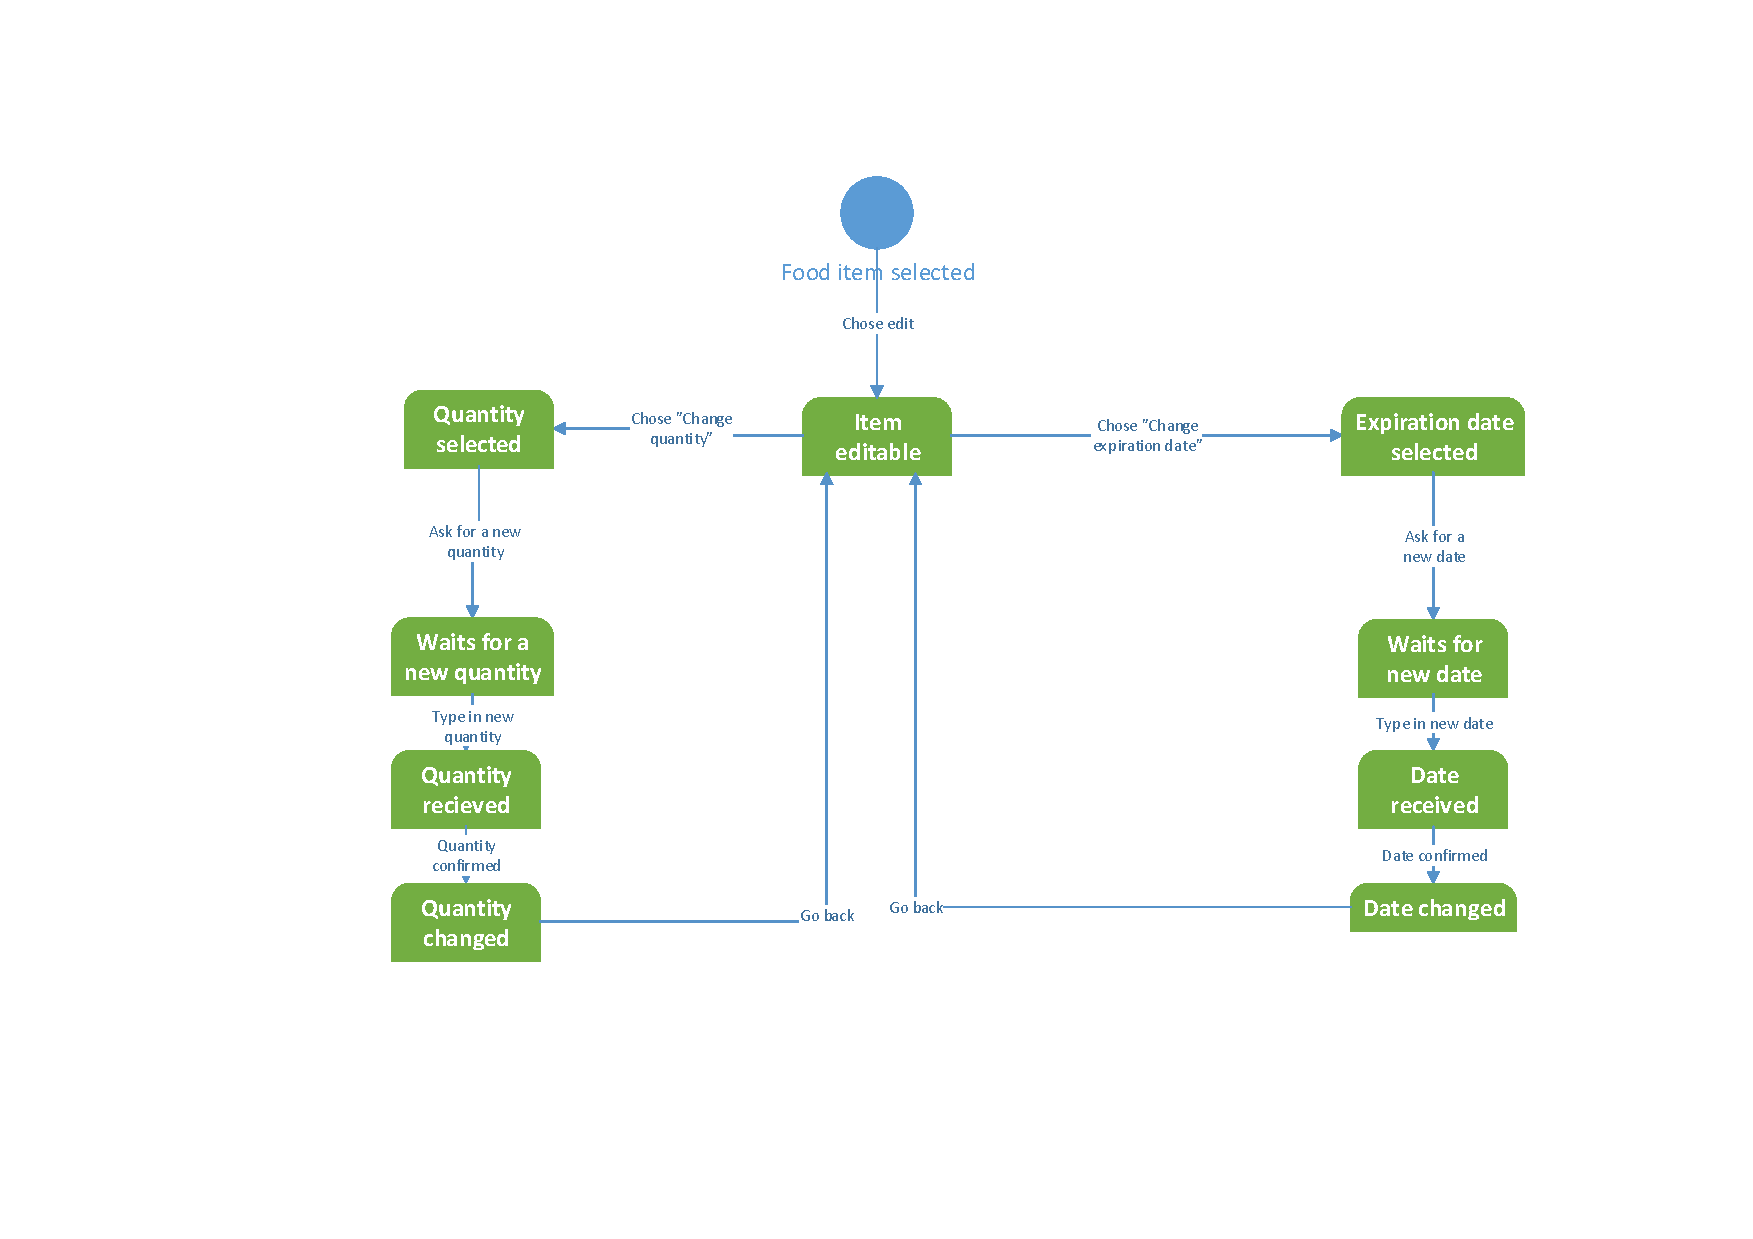
\includegraphics[width=1.0\textwidth, trim= 0 5cm 0 4cm]{ApplicationDomain/spEditInventory.pdf} 
	\caption{The \textit{Edit Inventory} state diagram.}
	\label{spEditInventory}
\end{figure}
The possible options in form of editing, is to change the quantity or expiration date. 
When choosing \textit{Change quantity} it works like the \textit{Change quantity} in the shopping list, which means that choosing an amount that leaves it at zero deletes the item, and leaving it below zero is not allowed. When the user tries to change the expiration date, the system prompts for a new date. All dates will be valid, which means that an item which was expired can go \textit{unexpired} as described at the diagram \cref{MealClass}. This also works the other way around as a fresh item can expire if the date changes to the day prior to the day it expires.

\subsection*{Summary}
The actor specification and use cases helped to establish an understanding of how the user base will interact with the system. By defining the use cases, some flaws in the design were discovered which resulted in varies corrections.